\section{Introdução}\label{sec:Introduction}

O projeto que se descreve neste relatório tem o objetivo de, utilizando os conhecimento adquiridos na componente prática de Administração e Exploração de Bases de Dados, construir um monitor web de uma BD Oracle. Para isto, foram necessários quatro passos bem distintos entre si e que se descrevem durante este relatório, em cada secção. O primeiro passo foi a extração dos dados das várias tabelas das várias bases de dados, o segundo passos foi o armazenamento destes dados em tabelas por nós criadas, o terceiro passo foi a criação de uma RESTful API em JSON e por último o desenvolvimento de uma aplicação web que permitisse a visualização interativa dos dados. A arquitetura concebida é a seguinte:
\vspace{5mm}
\begin{figure}[H]
    \centering
    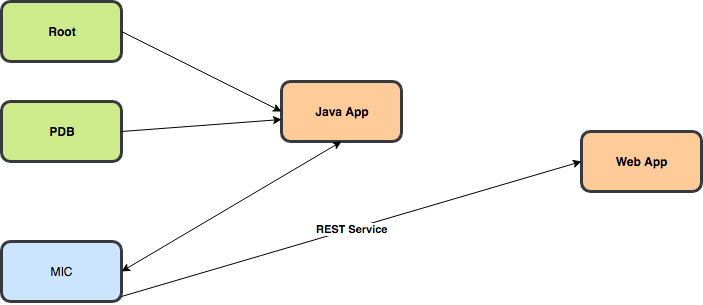
\includegraphics[scale=0.6]{tex/img/aebd.png}
    \caption{Arquitetura da aplicação}
    \label{fig:aa}
\end{figure}
